\section{742 --- Closest Leaf in a Binary Tree}
Given a binary tree \textbf{where every node has a unique value}, and a target key $k$, find the value of the nearest leaf node to target $k$ in the tree.

Here, nearest to a leaf means the least number of edges traveled on the binary tree to reach any leaf of the tree. Also, a node is called a leaf if it has no children.

In the following examples, the input tree is represented in flattened form row by row. The actual root tree given will be a \fcj{TreeNode} object.

\paragraph{Example 1:}
\begin{flushleft}


\textbf{Input}:

\fcj{root = [1, 3, 2]}, \fcj{k = 1}

Diagram of binary tree:

\begin{figure}[H]
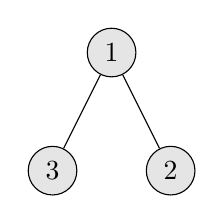
\begin{tikzpicture}
[every node/.style={draw, circle, fill=gray!20!, minimum size=5mm}]
\node{1}
child{node{3}}
child{node{2}};
\end{tikzpicture}
\end{figure}
%          1
%         / \
%        3   2

\textbf{Output}: 2 (or 3)

\textbf{Explanation}: Either 2 or 3 is the nearest leaf node to the target of 1.
\end{flushleft}

\paragraph{Example 2:}
\begin{flushleft}


\textbf{Input}:

\fcj{root = [1], k = 1}

\textbf{Output}: 1


\textbf{Explanation}: The nearest leaf node is the root node itself.
\end{flushleft}

\paragraph{Example 3:}
\begin{flushleft}

\textbf{Input}:

\fcj{root = [1,2,3,4,null,null,null,5,null,6]}, \fcj{k = 2}

Diagram of binary tree:

\begin{figure}[H]
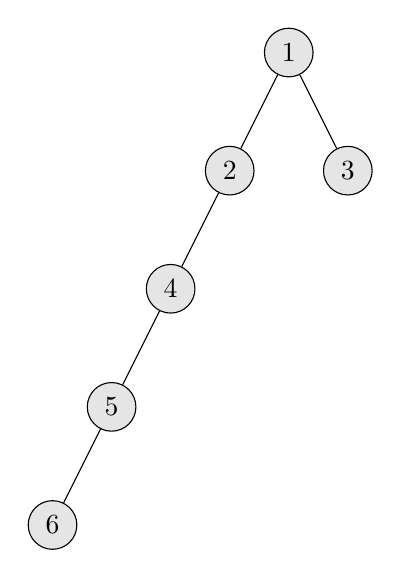
\begin{tikzpicture}
[every node/.style={draw, circle, fill=gray!20!, minimum size=5mm}]
\node{1}
child{node{2} child{node{4} child{node{5} child {node{6}} child[missing]} child[missing]} child[missing]}
child{node{3}};
\end{tikzpicture}
\end{figure}
%             1
%            / \
%           2   3
%          /
%         4
%        /
%       5
%      /
%     6

\textbf{Output}: 3

\textbf{Explanation}: The leaf node with value 3 (and not the leaf node with value 6) is nearest to the node with value 2.
\end{flushleft}

\paragraph{Note:}

\begin{itemize}
\item \fcj{root} represents a binary tree with at least 1 node and at most 1000 nodes.
\item Every node has a unique node.val in range \fcj{[1, 1000]}.
\item There exists some node in the given binary tree for which \fcj{node.val == k}.
\end{itemize}

\subsection{Covert To Graph}
If we can convert the binary tree into a graph, we can use breadth first search to obtain the closest node. In the graph, we do not have the concept of parent and child nodes. Hence, we need to add the parent of current node to its adjacent nodes.

First, we use \textit{DFS} to build the graph from the given tree. Then, we start from those nodes with value equal to $k$ to make \textit{BFS}. In order to avoid go through visited nodes, we make use of a hash set to record nodes we have checked.

\setcounter{lstlisting}{0}
\begin{lstlisting}[style=customc, caption={BFS On Graph Representation Of Binary Tree}]
int findClosestLeaf( TreeNode* root, int k )
{
    //convert tree to adjacent list graph
    unordered_map<TreeNode*, vector<TreeNode*>> g;
    build_graph( g, root, nullptr );
    //find closet leaf node using bfs
    //we need seen to record visited nodes
    queue<TreeNode*> q;
    unordered_set<TreeNode*> seen;
    for( auto const& [node, _] : g )
    {
        if( node->val == k )
        {
            q.push( node );
            seen.insert( node );
        }
    }
    //BFS
    while( !q.empty() )
    {
        auto t = q.front();
        q.pop();

        const auto& adjs = g[t];

        if( adjs.size() == 1 )
        {
            //only leaf node has only one neighbors
            return t->val;
        }
        //find in the adjacent nodes
        for( auto adj : adjs )
        {
            if( seen.find( adj ) == seen.end() )
            {
                seen.insert( adj );
                q.push( adj );
            }
        }
    }
    return k;
}
//helper recursive function to build graph from the binary tree
void build_graph( unordered_map<TreeNode*, vector<TreeNode*>>& G, TreeNode* node, TreeNode* parent )
{
    if( node )
    {
        auto p_node = G.find( node );
        if( p_node == G.end() )
        {
            p_node = G.emplace( node, vector<TreeNode*> {} ).first;
        }
        //add its parent (the parent maybe nullptr for root node)
        p_node->second.push_back( parent );
        if( parent )
        {
            auto p_par = G.find( parent );
            if( p_par == G.end() )
            {
                p_par = G.emplace( parent, vector<TreeNode*> {} ).first;
            }
            p_par->second.push_back( node );
        }
        //recursively build graph for left child
        build_graph( G, node->left, node );
        //recursively build graph for right child
        build_graph( G, node->right, node );
    }
}
\end{lstlisting}

\subsection{Get Distance To The Target Node}
We can make use of \textit{DFS} to find the node with target value. Then the closest leaf to this node must have a \textbf{lowest common ancestor} with the node. Also, this ancestor is on the path from the \fcj{root} to this target node. 

We can get the distances of all ancestors to the target node during \textit{DFS} process via a hash map. Then, we traverse the binary tree. For each node, we check if this node is one of ancestor of the target node through the hash map. If this ancestor is a leaf node, compare against current minimum distance and update result node and minimum distance so far accordingly.

\begin{lstlisting}[style=customc, caption={Get Distances}]
{
    unordered_map<TreeNode*, int> dists;
    //find the ancestor nodes
    //that in the path from root to target node
    find_k( root, k, dists );
    //DFS: get the closest node
    int min_dist = 100000000;
    int ans = k;
    search( root, dists, -1, min_dist, ans );
    return ans;
}
//helper function to find the ancestor nodes from root to the target node
//and get the distance to the target node
int find_k( TreeNode* t, int k, unordered_map<TreeNode*, int>& dists )
{
    //invalid node
    if( !t )
    {
        return -1;
    }
    if( t->val == k )
    {
        //the target node
        dists[t] = 0;
        return 0;
    }
    auto d = find_k( t->left, k, dists );
    if( d != -1 )
    {
        //we find the target node in the left child tree
        //since all nodes have unique values
        //we can return from here
        //1 means the distance from t to t->left
        dists[t] = 1 + d;
        return 1 + d;
    }
    //target node does not exist in the left child tree
    //find in the right child tree
    d = find_k( t->right, k, dists );
    if( d != -1 )
    {
        //1 means the distance from t to t->left
        dists[t] = 1 + d;
        return 1 + d;
    }
    //target node doesn't exist in t's child tree
    return -1;
}
//hepler function to find closest leaf node
void search( TreeNode* t, unordered_map<TreeNode*, int>& dists, int dist, int& min_dist, int& closest )
{
    if( !t )
    {
        return;
    }
    auto p = dists.find( t );
    if( p != dists.end() )
    {
        //get the distance from current node to the target node
        //from the recorded dists
        dist = p->second;
    }
    //check if this node is a leaf node
    if( !t->left && !t->right )
    {
        //check if this leaf node
        //has shortest disance
        //to the target node
        if( dist < min_dist )
        {
            min_dist = dist;
            closest = t->val;
        }

        return;
    }
    //search in the left child tree
    search( t->left, dists, dist + 1, min_dist, closest );
    //search in the right child tree
    search( t->right, dists, dist + 1, min_dist, closest );
}
\end{lstlisting}
